\documentclass{article}
\usepackage[LGR,T1]{fontenc}
\usepackage[utf8]{inputenc}
\usepackage[greek, english]{babel}
\usepackage{alphabeta}
\usepackage{natbib}
\usepackage{graphicx}
\usepackage{biblatex}
\usepackage{hyperref}
\usepackage{tabularx}

\addbibresource{references.bib}

\def\code#1{\texttt{#1}}

\usepackage{eso-pic}% http://ctan.org/pkg/eso-pic
\usepackage{lipsum}% http://ctan.org/pkg/lipsum

\title{Project Plan-v0.1}

\author{\\

\includegraphics[width=3in]{safeguard}\\[1ex]\\\\
}

\begin{document}

\maketitle

\newpage


Θεόδωρος Ντάκουρης - ntakouris@ceid.upatras.gr - ΑΜ 1054332 : Editor 


Νίκος Σουλτάνης - soultanis@ceid.upatras.gr - ΑΜ 1054319 : Contributor & Reviewer

\renewcommand{\contentsname}{Περιεχόμενα}
\tableofcontents

\clearpage
\section{Χρονοπρογραμματισμός}
\subsection{Gantt Chart}

\begin{center}
 \makebox[\textwidth]{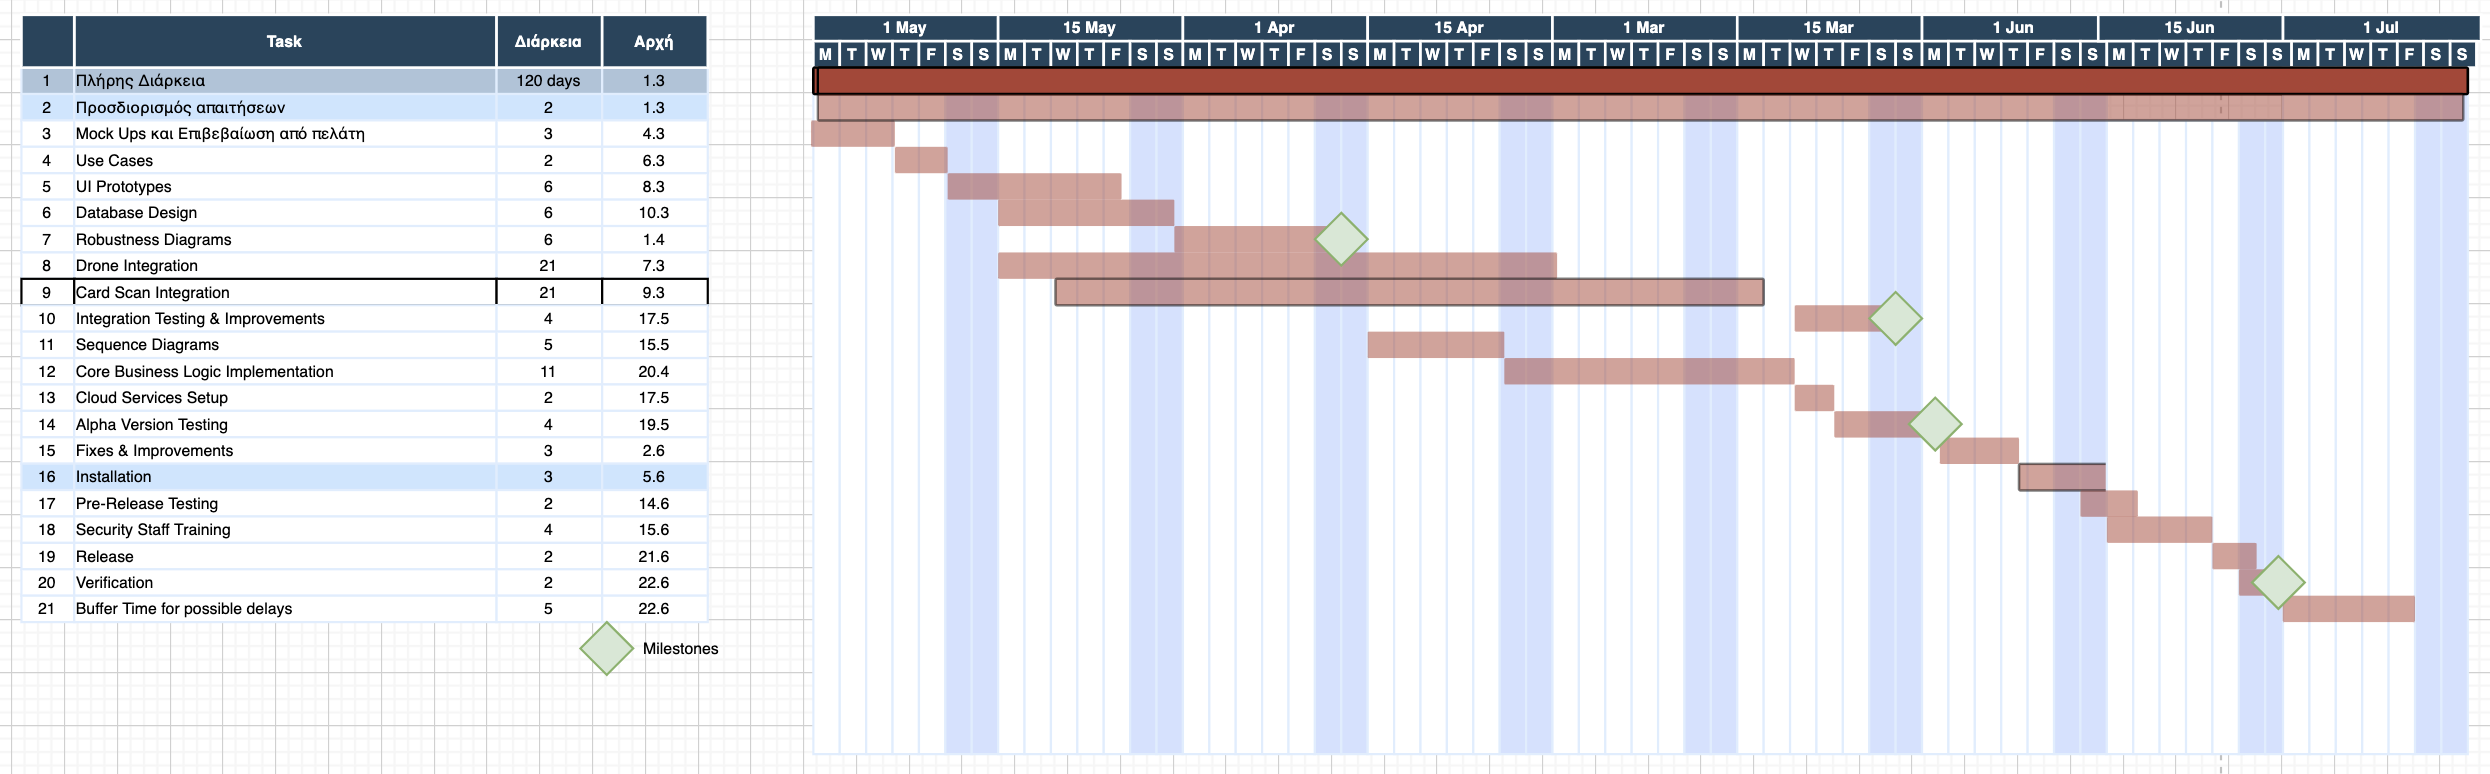
\includegraphics[width=.9\paperwidth]{gant.png}}
\end{center}
\subsection{Pert Chart}
\begin{center}
 \makebox[\textwidth]{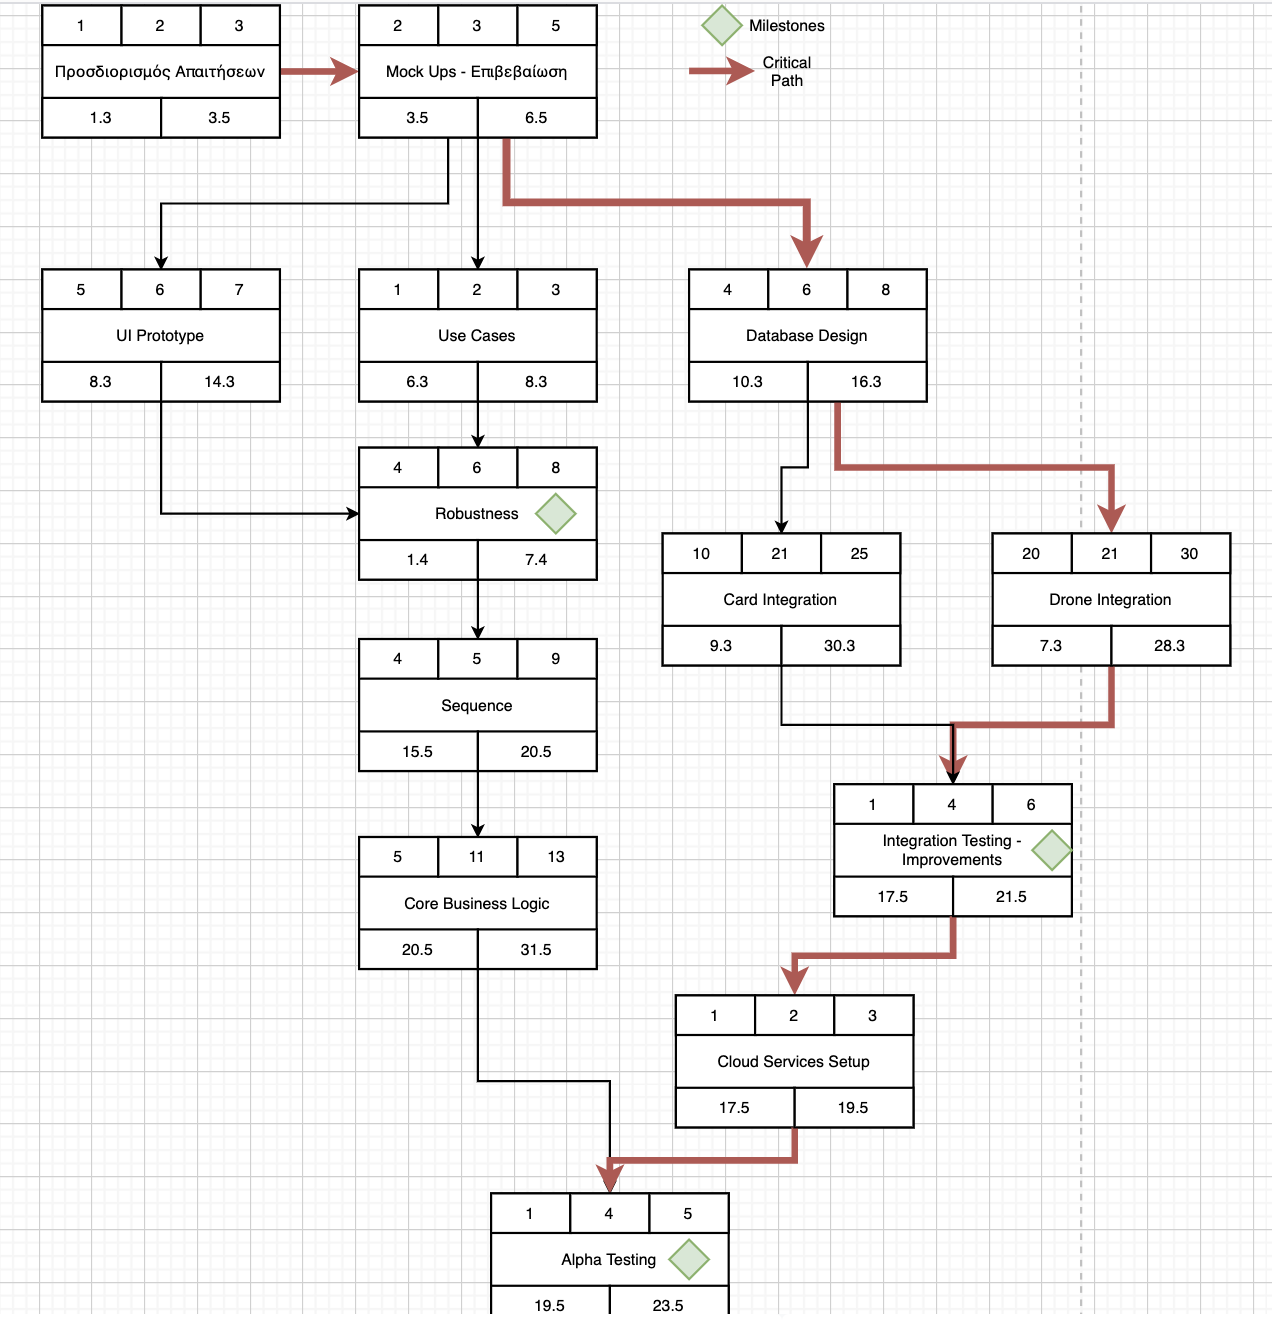
\includegraphics[width=\paperwidth]{pert-1.png}}

\centering
 \makebox[\textwidth]{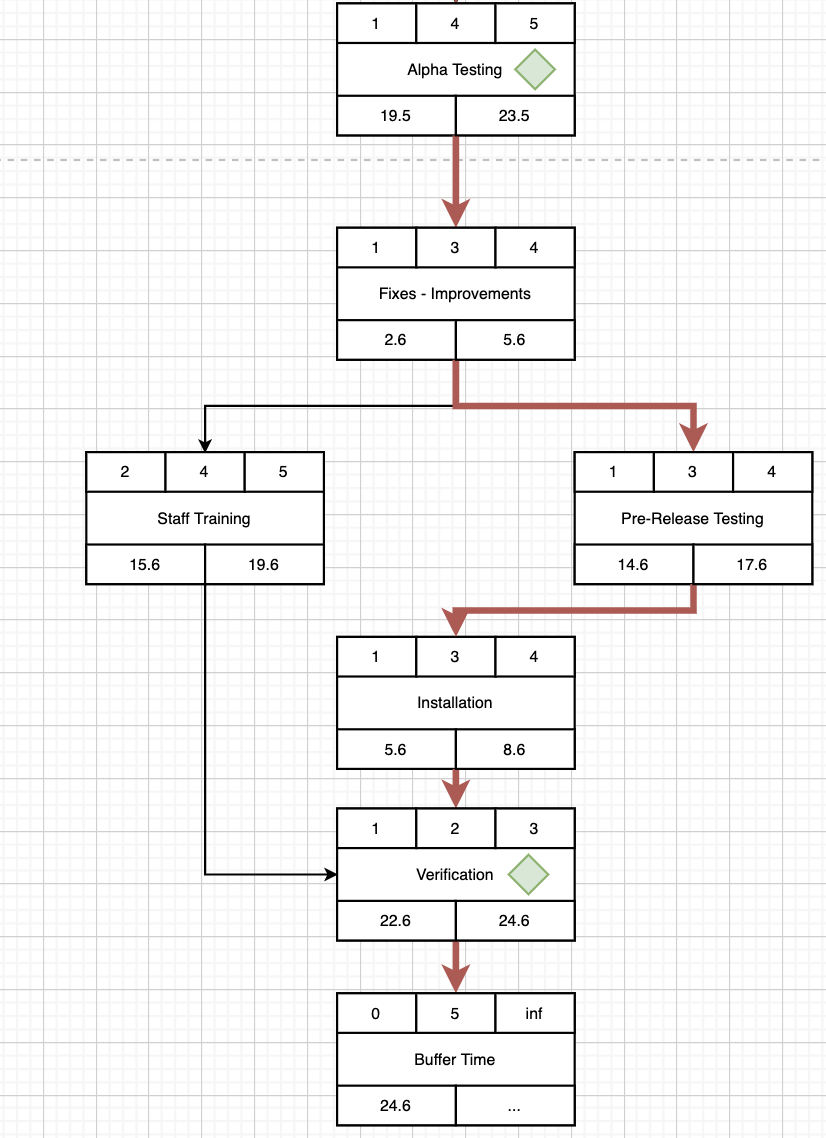
\includegraphics[width=.8\paperwidth]{pert-2.png}}
\end{center}

\section{Καταμέριση Εργασίας}

Όπως φαίνεται στο Gantt-Pert Chart, σκοπεύουμε να έχουμε παραδόσει το έργο μια εβδομάδα πιο πριν από τη συμφωνημένη ημερομηνία ώστε να έχουμε χρόνο να προλάβουμε τυχόν καθυστερήσεις ή προβλήματα που μπορεί να προκύψουν.

Θεωρούμε πως χρησιμοποιούμε κάποιο έτοιμο πακέτο για κάρτες και scanning καθώς και για drones κάποιο έτοιμο πακέτο που δεν χρειάζεται hardware infrastructure από εμάς, όπως το \href{https://www.skydio.com/}{Skydio}. 

Η καταμέριση μικρών task σε κάθε έναν θα είναι ως εξής:

\noindent\begin{tabularx}{\hsize}{||l|l|l|l|l|l||}
\hline
    Task & Ντάκουρης & Σουλτάνης & Λασκαρέλιας & Πάπα & Βασιλόπουλος \\
    \hline
        Απαιτήσεις & x & x & x & x  & x \\
        Mock ups & x & x & x & x  & x \\
        Επιβεβαίωση & x & x & x & x  & x \\
        Use Cases &&&x&x& \\
        UI Prototype &&x&x&& \\
        DB Design x & x &&&& \\
        Robustness & x & & & x & x\\
        Drones & & x & x & x & \\
        Card Scan & x & & & x & \\
        Integration Test & x & x & x & x & x \\
        Improvements & x & & & x & \\
        Sequence & & & x& & x\\
        Business Logic & x & x &&& \\
        Cloud Setup & x & & & & \\
        Alpha Test & x & x & x & x & x \\
        Installation & x & x & & x &\\ 
        Pre-Release Test &  &  & & x & x\\ 
        Staff Training & & x & x &  & x \\
        Release & x & x & x & x & x \\
        Verification & x & x & x & x & x \\
\hline

\end{tabularx}

\\
Μπορεί να χρειαστεί να προσλάβουμε κάποιον junior software engineer για να φτιάξει την ιστοσελίδα ή για επιπλέον field work καθώς (τα θεωρούμε σχετικά απλά tasks) καθώς και κάποιον δικηγόρο ή λογιστή περιστασιακά για δημιουργία εταιρίας και συμβόλαια πώλησης.

\section{Κόστος}

Οι 'μισθοί' του κάθε μέλους (ατομικά έξοδα δηλαδή) θα ανέρχονται στα 1000 ευρώ το μήνα καθαρά συν 200 ευρώ (1200 μεικτά). Θα χρησιμοπιήσουμε το μεγάλο σπίτι του Βάιου μέχρι να κάνουμε την πρώτη πώληση και να μεταφερθούμε σε γραφείο. Υπολογίζουμε πως τα μηνιαία έξοδα του σπιτιού είναι στα 1000 ευρώ μηνιαία συμπεριλαμβάνοντας τυχόν utilities, καφέδες και φαγητό. Τα δικηγορικά και λογιστικά έξοδα τα περιμένουμε να είναι γύρω στα 2000-3000 μέχρι και την πρώτη πώληση. Τα κόστη των server είναι στα 10 ευρώ το μήνα μέχρι να αποκτήσουμε αρκετό scale που θα ανεβεί ανάλογα με το traffic. Θα χρησιμοποιήσουμε κάποιο managed cloud όπως AWS/GCP/Azure για να μην έχουμε τέτοια προβλήματα με scaling. Έξτρα hardware που περιλαμβάνει 2 drones για testing και ένα development kit καρτών κοστίζουν συνολικά 2500 ευρώ.

Άρα συνολικα, υπολογίζουμε το κόστος να είναι στα 7-9 χιλιάρικα (ελαφρώς αισιόδοξα πως θα έχουμε τελειώσει σε 6 μήνες).

Η τιμή πώλησης του κάθε project εξαρτάται από το μέγεθος και τις έξτρα απαιτήσεις (επιπλέον drones, κάρτες ή on-premises servers) του κάθε πελάτη.

\section{Εργαλεία}
Χρησιμοποιήθηκαν:
\begin{itemize}
    \item \LaTeX/Overleaf.com - Συγγραφή του παρόντος τεχνικού κειμένου
    \item Photoshop - Φωτογραφία Σελίδας Τίτλου
    \item draw.io - Mock Up Wireframes, Pert, Gantt Charts
\end{itemize}


\end{document}
